\documentclass[notitlepage]{report}
\usepackage{graphicx}
\usepackage{amsmath}
\usepackage{amssymb}
\usepackage[parfill]{parskip}
\newcommand\numberthis{\addtocounter{equation}{1}\tag{\theequation}}
\usepackage{titling}
\usepackage{listings}
\usepackage{xcolor}


\lstdefinestyle{mystyle}{
    backgroundcolor=\color{white},   
    breakatwhitespace=false,         
    breaklines=true,                 
    captionpos=b,                    
    keepspaces=true,                 
    showspaces=false,                
    showstringspaces=false,
    showtabs=false,                  
    tabsize=2,
    framextopmargin=3pt,  
    framexbottommargin=3pt
}
\lstset{frame=lines}
\lstset{style=mystyle}

\title{Desmos Polygonal Number Diagrams}
\author{Dan MacKinnon}

\begin{document}
\maketitle
\begin{abstract}
\noindent
Polygonal numbers, like the triangular, square, and pentagonal numbers, are closely identified with (or even defined in terms of) the diagrams that they are associated with. The functional programming capabilities of the Desmos graphing calculator provides fun and interesting ways of exploring number diagrams like those associated with polygonal numbers. This short article provides one approach that can be used to build polygonal number diagrams in Desmos.  
\end{abstract}

\section*{Polygonal numbers}
For a given $k \in \mathbb{Z}^+, k>2$, the $k$-polygonal numbers are a recursively defined integer sequence, as shown in Equation (\ref{eq:defn1}). 

\begin{align*}
    p_{k, 1} &= 1 \\
    p_{k,i} &= p_{k,i-1} + (k-2)i - (k-3)
    \numberthis
    \label{eq:defn1}
\end{align*}

For a term in the sequence $n = p_{k,i}$, $n$ dots can be arranged in a regular $k$-polygon built up of $i$ layers (traditionally referred to as \textit{gnomons}), as shown for the pentagonal numbers ($k=5$) of Figure (\ref{fig:pentagonals}). 

\begin{figure}[!htb]
    \centering
    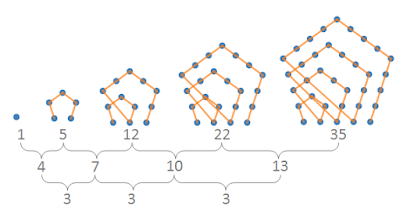
\includegraphics[width=0.5\linewidth]{pentagonal_numbers.PNG}
    \caption{The first few pentagonal numbers, showing first and second differences}
    \label{fig:pentagonals}
\end{figure}

If $n$ is the $i$th $k$-polygonal number, it can be drawn as a layered regular $k$-polygon with $i$ gnomon layers, as shown for the third pentagonal number $12$, $p_{5,3}=12$, in Figure (\ref{fig:gnomons}.

\begin{figure}[!htb]
    \centering
    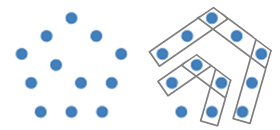
\includegraphics[width=0.5\linewidth]{pentagon_with_gnomon.PNG}
    \caption{Pentagonal number diagram $n=12$ with gnomons}
    \label{fig:gnomons}
\end{figure}

\section*{Placing any $n$ in a $k$-polygonal diagram}

Let $n,k \in \mathbb{Z}^{+}$, $k > 2$. We would like to draw the $k-$polygonal number diagram ``up to'' $n$. If $n$ happens to actually be a $k-$polygonal number, this will be a complete diagram with $n$ dots in a layered $k$-polygon. Otherwise, this will be a diagram whose outer gnomon layer is incomplete.

Figure (\ref{fig:hexagonals}) shows hexagonal number ($k = 6$) diagrams for the numbers 15 and 26. Because 15 actually is a hexagonal number, the diagram is complete. The diagram for 26 shows an incomplete diagram, with an incomplete outer layer.

\begin{figure}[!htb]
    \centering
    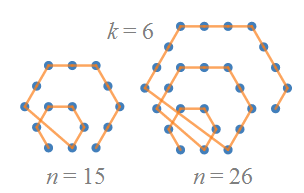
\includegraphics[width=0.5\linewidth]{hexagonal_and_no.PNG}
    \caption{Two hexagonal diagrams ($k = 6$), 15 is hexagonal, 26 is not}
    \label{fig:hexagonals}
\end{figure}


\subsection*{Finding the gnomon for $n$ and $k$}

The recursive definition for $p_{k,1}$ in Equation (\ref{eq:defn1} yields formulas stated as a summation (\ref{eq:summation}) and a direct calculation (\ref{eq:quad}).

\begin{equation}
    p_{k,i} = \sum^{i}_{j=1}\left[(k-2)j-(k-3)\right]
    \label{eq:summation}
\end{equation}

\begin{equation}
    p_{k,i} = \frac{(k-2)i(i+1)}{2} - (k-3)i
    \label{eq:quad}
\end{equation}

Applying the quadratic formula to solve $n-p_{k,i}=0$ provides us with

\begin{equation}
    g\left(n,k\right)=\frac{\left(k-4\right)+\sqrt{\left(k-4\right)^{2}+8n\left(k-2\right)}}{2\left(k-2\right)}
     \label{eq:quadform}
\end{equation}

This allows us to identify the gnomon layer $\text{gnomon}(n,k)$ that a given $n$ will sit in within a $k$-polygonal diagram (\ref{eq:gnomon}).

\begin{equation}
    \text{gnomon}\left(n,k\right) = \text{ceil}\left(g\left(n\right)\right)  
    \label{eq:gnomon}
\end{equation}

\subsection*{The position of $n$ within its gnomon layer}

The size of the gnomon layer that $n$ will sit in (how many dots would be in the layer within the diagram) is given by Equation (\ref{eq:gnomon-size}).

\begin{equation}
\text{gsize}\left(n,k\right)= 1+(\text{gnomon}\left(n,k\right)-1)\cdot\left(k-2\right)
\label{eq:gnomon-size}
\end{equation}

To find the position of the $n$th dot within the gnomon, we need to count the number of dots that came before it within that gnomon. To do this we can sum up to $n-1$ over a function whose value is $0$ for all $i$ where $gnomon(i,k)<gnomon(n,k)$, and whose value is $1$ for those $i$ where $gnomon(i,k)=gnomon(n,k)$. This sum that gives us the "depth" of \textit{n} within its gnomon is provided by Equation (\ref{eq:gnomon-depth}).

\begin{equation}
    \text{gdepth}\left(n,k\right)=\sum_{i=1}^{n}\left(\text{floor}\left(\frac{gnomon\left(i,k\right)}{gnomon\left(n,k\right)}\right)\right)
    \label{eq:gnomon-depth}
\end{equation}

\section*{Drawing the diagram}

For a given $n,k \in \mathbb{Z}^{+}$, $k > 2$, the preceding sections tell us which gnomon $n$ will be placed in in a $k$-polygonal diagram, and in which spot along the gnomon. 

To complete the diagram, we need to also determine how much the gnomon is bent at the particular position that $n$ finds itself at. Because the gnomon is a layer in a regular $k$-gon, it bends in increments of the base angle $alpha_k$ that is given by Equation (\ref{eq:angle}).


\begin{equation}
    \alpha_k=\left(\pi-((k-2)*(\pi/k))\right)
\label{eq:angle}
\end{equation}

As we draw a gnomon, we'll start at the left-most position, which for a given $n$ can be expressed by $(x_0(n,k),y_0(n,k)$ as defined in (\ref{eq:init-points}).

\begin{align*}
    x_0\left(n,k\right) &= -\text{gnomon}\left(n,k\right)\cos{(\alpha_k)} \\
    y_0\left(n,k\right) &=
    \text{gnomon}\left(n,k\right)\sin{(\alpha_k)} 
    \numberthis
    \label{eq:init-points}
\end{align*}

Starting at the initial point $(x_0(n,k),y_0(n,k)$ for a given $n$, we want to move along the gnomon layer up to the gnomon depth of $n$ ($\text{gdepth}(n)$), bending along the gnomon as required. This process is expressed by the sums in the definitions of $x(n,k)$ and $y(n,k)$ of (\ref{eq:all}).

\begin{align*}
x(n,k) &= x_0(n,k) - \sum_{j=1}^{\text{gdepth}\left(n\right)-1}\cos\left(\alpha_{k}\cdot\left[\operatorname{ceil}\left(\frac{j}{\text{gsize}\left(n\right)}\left(k-2\right)\right)+1\right]\right)\\
\\
y(n,k) &= y_0(n,k) + \sum_{j=1}^{\text{gdepth}\left(n\right)-1}\sin\left(\alpha_k\cdot\left[\operatorname{ceil}\left(\frac{j}{\text{gsize}\left(n\right)}\left(k-2\right)\right)+1\right]\right)
\numberthis
\label{eq:all}
\end{align*}

\section*{Building in Desmos}

To begin building the polygonal number diagrams in Desmos, begin with creating sliders for $n$ and $k$, and a sequence $N$ of the integers between $1$ and $n$. The base angle can also be defined.

\begin{lstlisting}[escapeinside={(*}{*)}]
Slider (*$n$*); (*$1 \leq n \leq 100$*) step: (*10*)
Slider (*$k$*); (*$2 \leq k \leq 100$*) step: (*10*)
(*$N=\left[1,\ ...\ ,n\ \right]$*)
(*$a_{ngle}=\pi-(k-2)\cdot\frac{\pi}{k}$*)
\end{lstlisting}

Chose a variable name that does not correspond to one of the already used variables, and implement equations (\ref{eq:quadform}) and (\ref{eq:gnomon}). The value of $k$ is defined globally and does not need to be passed as a paramenter. The value of $n$ is not used directly; instead, the functions will be evaluated using the values of the array $N$. Here $l$ will be used as the parameter name rather than $n$. 

\begin{lstlisting}[escapeinside={(*}{*)}]
(*$g(l)=(k-4)+\text{sqrt}((k-4)^{2}+8l(k-2))/(2(k-2))$*)
\end{lstlisting}

\begin{lstlisting}[escapeinside={(*}{*)}]
(*$g_{nomon}(l) = \text{floor}(g(l))$*)  
\end{lstlisting}

Next, implement the gnomon size and depth functions.

\begin{lstlisting}[escapeinside={(*}{*)}]
(*$ g_{size}(l)= 1 +(g_{nomon}(l) - 1)\cdot(k-2)$*)
\end{lstlisting}

\begin{lstlisting}[escapeinside={(*}{*)}]
(*$g_{depth}(l)=\sum_{i=1}^{l}(\text{floor}(g_{nomon}(i)/g_{nomon}(l)))$*)
\end{lstlisting}

Finally, the equations for the coordinates of each plotted point can be defined based on equations (\ref{eq:init-points}) and (\ref{eq:all}).


\begin{lstlisting}[escapeinside={(*}{*)}]
(*$x_0(l) = -g_{nomon}(l)\cos{(a_{ngle})}$*)
(*$y_0(l)) = g_{nomon}(l)\sin{(a_{ngle})}$*)
\end{lstlisting}


\begin{lstlisting}[escapeinside={(*}{*)}]
(*$x_{poly}(l) = x_0(l) - \sum_{j=1}^{g_{depth}(l)-1}\cos(a_{ngle}\cdot(\operatorname{ceil}(({j}/{g_{size}(l)})(k-2))+1)) $*)

(*$y_{poly}(l) = y_0(l) - \sum_{j=1}^{g_{depth}(l)-1}\sin(a_{ngle}\cdot(\operatorname{ceil}(({j}/{g_{size}(l)})(k-2))+1)) $*)
\end{lstlisting}

To plot the points, the functions above are applied to the sequence $N$. The grid and axis can be removed from the plot.

\begin{lstlisting}[escapeinside={(*}{*)}]
(*$(x_{poly}(N),y_{poly}(N))$*)
\end{lstlisting}



\end{document}
